% -----------------------------------------------
% Template for ISMIR Papers
% 2016 version, based on previous ISMIR templates

% Requirements :
% * 6+1 page length maximum
% * 2MB maximum file size
% * Copyright note must appear in the bottom left corner of first page
% (see conference website for additional details)
% -----------------------------------------------

\documentclass{article}
\usepackage{ismir,amsmath,cite}
\usepackage{graphicx}
\usepackage{color}

% Title.
% ------
\title{Modulo7 : A full stack Music Information Retrieval And Structured Querying Engine}

% Note: Please do NOT use \thanks or a \footnote in any of the author markup

% Single address
% To use with only one author or several with the same address
% ---------------
%\oneauthor
% {Names should be omitted for double-blind reviewing}
% {Affiliations should be omitted for double-blind reviewing}

% Two addresses
% --------------
%\twoauthors
%  {First author} {School \\ Department}
%  {Second author} {Company \\ Address}

%% To make customize author list in Creative Common license, uncomment and customize the next line
%  \def\authorname{First Author, Second Author} 


% Three addresses
% --------------
\threeauthors
  {First Author} {Affiliation1 \\ {\tt author@ismir.edu}}
  {Second Author} {\bf Retain these fake authors in\\\bf submission to preserve the formatting}
  {Third Author} {Affiliation3 \\ {\tt author3@ismir.edu}}

%% To make customize author list in Creative Common license, uncomment and customize the next line
%  \def\authorname{First Author, Second Author, Third Author} 

% Four or more addresses
% OR alternative format for large number of co-authors
% ------------
%\multauthor
%{First author$^1$ \hspace{1cm} Second author$^1$ \hspace{1cm} Third author$^2$} { \bfseries{Fourth author$^3$ \hspace{1cm} Fifth author$^2$ \hspace{1cm} Sixth author$^1$}\\
%  $^1$ Department of Computer Science, University , Country\\
%$^2$ International Laboratories, City, Country\\
%$^3$  Company, Address\\
%{\tt\small CorrespondenceAuthor@ismir.edu, PossibleOtherAuthor@ismir.edu}
%}
%\def\authorname{First author, Second author, Third author, Fourth author, Fifth author, Sixth author}


\sloppy % please retain sloppy command for improved formatting

\begin{document}

%
\maketitle
%
\begin{abstract}
This paper describes a novel Music Information Retrieval and Structured Querying framework named Modulo7. Modulo7 is a full stack implementation (both client and server side software) which facilitates indexing variegated sources of music (midi, mp3, music xml and digitized sheet music files). Modulo7 implements a similarity search engine based on customized vector space representations of songs, an efficient indexing and persistent storage mechanism and an interface for querying attributes based on SQL(Structured Querying Language) like principles. The papers describes the implementation details and outlines speed up and scale up results over input sources and other MIR frameworks. \\\\
\textbf{Keywords : MIDI, Music XML, MP3, Music Retrieval, SQL}
\end{abstract}
%
\section{Introduction}\label{sec:introduction}

Given the explosive growth of Music Information Retrieval research, several approaches and software suits have been designed to tackle generic problems such as efficient indexing, similarity searches, archival methods, structured and un-structured querying ,feature extraction, audio and digital signal processing. A vast majority of the MIR frameworks in academia tend to approach very specific problems and does not support scalability as a significant end goal in itself \cite{mirproblems}. Moreover, industry applications predominantly treat MIR applications based on collaborative filtering approaches \cite{amazonreco} and/or manual annotation \cite{musicgenomepandora} instead of structural analysis of music sources yet scales very well to large datasets. \\\\
Modulo7 is an attempt to capture the best features of both worlds. Modulo7 converts different music sources (midi, musicxml files, sheet music png/jpeg files and mp3) into a single unified symbolic representation. It indexes songs on different properties (artist, key signature, time signature etc). 

%
\section{Relevant Work} \label{sec:relevantwork}

Music Information Retrieval is a vast and interdisciplinary body of work. In order to facilitate research in MIR, several software suits and frameworks have been developed in the past. Notable amongst them are software suits like jMIR \cite{jMIR} for automatic feature extraction from audio and midi sources, marsyas \cite{marsyas} and essentia \cite{essentia} for audio processing, humdrum \cite{humdrum} for automated musicological research, gamera \cite{gamera} for optical music recognition, 

\section{Modulo7 Architecture and Design}\label{sec:architecture}

This section details the software architecture of the Modulo7. The Modulo7 architecture can be visualized as \ref{fig:architecture} and is broadly divided into the following components 

\begin{enumerate}
\item \textbf{Music parsers: } Components that individually parse different music sources into a unified symbolic representation. as described in \ref{fig:document}
\end{enumerate}

\begin{figure}
 \centerline{\framebox{
 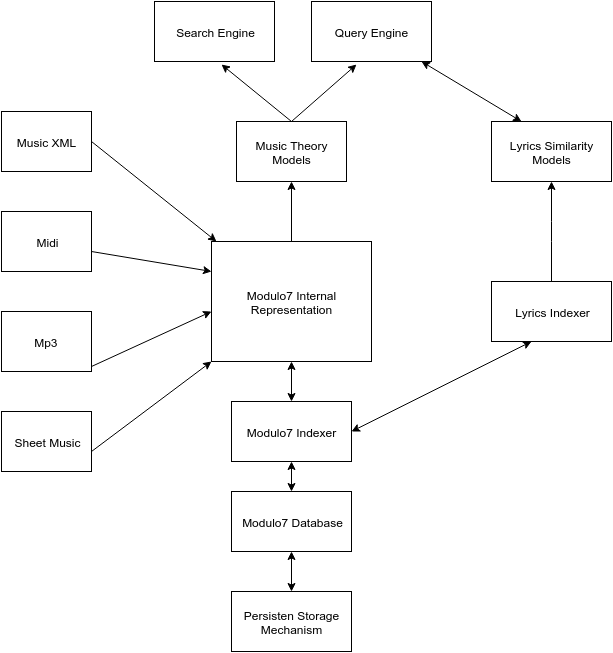
\includegraphics[width=\columnwidth]{Modulo7Architecture.png}}}
 \caption{A block diagram of the Modulo7 Architecture.}
 \label{fig:architecture}
\end{figure}

\begin{figure}
 \centerline{\framebox{
 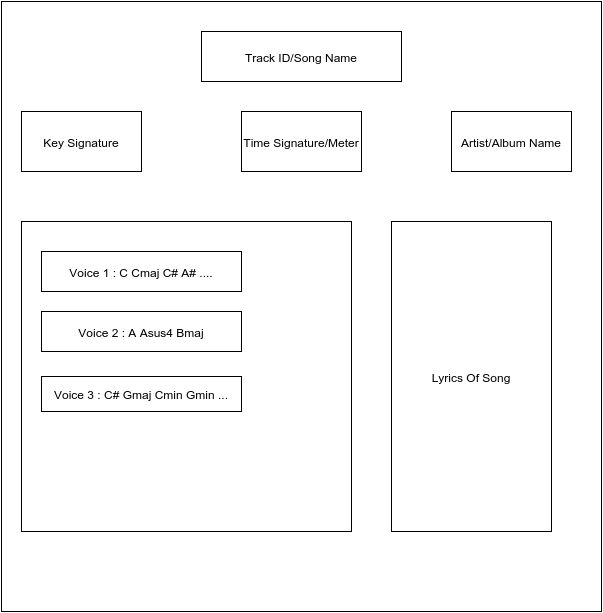
\includegraphics[width=\columnwidth]{DocumentStructureOfModulo7.png}}}
 \caption{Figure captions should be placed below the figure.}
 \label{fig:document}
\end{figure}

\section{Typeset Text}\label{sec:typeset_text}

\subsection{Normal or Body Text}\label{subsec:body}

Please use a 10pt (point) Times font. Sans-serif or non-proportional fonts
can be used only for special purposes, such as distinguishing source code text.

The first paragraph in each section should not be indented, but all other paragraphs should be.

\subsection{Title and Authors}

The title is 14pt Times, bold, caps, upper case, centered.
Authors' names are omitted when submitting for double-blind reviewing.
The following is for making a camera-ready version.
Authors' names are centered.
The lead author's name is to be listed first (left-most), and the co-authors' names after.
If the addresses for all authors are the same, include the address only once, centered.
If the authors have different addresses, put the addresses, evenly spaced, under each authors' name.

\subsection{First Page Copyright Notice}

Please include the copyright notice exactly as it appears here in the lower left-hand corner of the page.
It is set in 8pt Times.

\subsection{Page Numbering, Headers and Footers}

Do not include headers, footers or page numbers in your submission.
These will be added when the publications are assembled.

\section{First Level Headings}

First level headings are in Times 10pt bold,
centered with 1 line of space above the section head, and 1/2 space below it.
For a section header immediately followed by a subsection header, the space should be merged.

\subsection{Second Level Headings}

Second level headings are in Times 10pt bold, flush left,
with 1 line of space above the section head, and 1/2 space below it.
The first letter of each significant word is capitalized.

\subsubsection{Third and Further Level Headings}

Third level headings are in Times 10pt italic, flush left,
with 1/2 line of space above the section head, and 1/2 space below it.
The first letter of each significant word is capitalized.

Using more than three levels of headings is highly discouraged.

\section{Footnotes and Figures}

\subsection{Footnotes}

Indicate footnotes with a number in the text.\footnote{This is a footnote.}
Use 8pt type for footnotes. Place the footnotes at the bottom of the page on which they appear.
Precede the footnote with a 0.5pt horizontal rule.

\subsection{Figures, Tables and Captions}

All artwork must be centered, neat, clean, and legible.
All lines should be very dark for purposes of reproduction and art work should not be hand-drawn.
The proceedings are not in color, and therefore all figures must make sense in black-and-white form.
Figure and table numbers and captions always appear below the figure.
Leave 1 line space between the figure or table and the caption.
Each figure or table is numbered consecutively. Captions should be Times 10pt.
Place tables/figures in text as close to the reference as possible.
References to tables and figures should be capitalized, for example:
see \figref{fig:example} and \tabref{tab:example}.
Figures and tables may extend across both columns to a maximum width of 17.2cm.

\begin{table}
 \begin{center}
 \begin{tabular}{|l|l|}
  \hline
  String value & Numeric value \\
  \hline
  Hello ISMIR  & \conferenceyear \\
  \hline
 \end{tabular}
\end{center}
 \caption{Table captions should be placed below the table.}
 \label{tab:example}
\end{table}

\section{Equations}

Equations should be placed on separate lines and numbered.
The number should be on the right side, in parentheses, as in \eqnref{relativity}.

\begin{equation}\label{relativity}
E=mc^{2}
\end{equation}

\section{Citations}

All bibliographical references should be listed at the end,
inside a section named ``REFERENCES,'' numbered and in alphabetical order.
All references listed should be cited in the text.
When referring to a document, type the number in square brackets
\cite{Author:00}, or for a range \cite{Author:00,Someone:10,Someone:04}.

% For bibtex users:
\bibliography{ISMIRtemplate}

% For non bibtex users:
%\begin{thebibliography}{citations}
%
%\bibitem {Author:00}
%E. Author.
%``The Title of the Conference Paper,''
%{\it Proceedings of the International Symposium
%on Music Information Retrieval}, pp.~000--111, 2000.
%
%\bibitem{Someone:10}
%A. Someone, B. Someone, and C. Someone.
%``The Title of the Journal Paper,''
%{\it Journal of New Music Research},
%Vol.~A, No.~B, pp.~111--222, 2010.
%
%\bibitem{Someone:04} X. Someone and Y. Someone. {\it Title of the Book},
%    Editorial Acme, Porto, 2012.
%
%\end{thebibliography}

\end{document}
